% vim: set tw=78 sts=2 sw=2 ts=8 aw et ai:
\documentclass[conference]{IEEEtran}

%\usepackage{ucs}
\usepackage{url}
%\usepackage[utf8x]{inputenc}
\usepackage[english]{babel}
%\usepackage{hyperref}	  % use \url{http://$URL} or \href{http://$URL}{Name}
\usepackage{underscore}	  % underscores need not be escaped
%\usepackage{subfigure}
\usepackage{verbatim}
\usepackage{float}
\usepackage{amsmath, amsthm, amssymb}
\usepackage{parskip}
%\usepackage{flushend}

% Support for including graphics
\usepackage{graphicx}
\DeclareGraphicsExtensions{.pdf,.png,.jpg}

\begin{document}

\title{Diagram generation using genetic layout algorithms and orthogonal routing}



\author{
\IEEEauthorblockN{Andrei Musat, Andrei Voinescu}
\IEEEauthorblockA{
  Automatic Control and Computers Faculty\\
  University Politehnica of Bucharest,\\
  \{andrei.musat@cti.pub.ro, andrei.voinescu@cs.pub.ro\}}
  }

\maketitle

\begin{abstract} 
Wireless sensor networks are a cheap and versatile solution for monitoring various environments 
and elements of an environment. There exists a number of such applications used worldwide to monitor 
areas in which human access is hard or near impossible. The issue with these applications is that 
they are mainly used by government organizations or for research purposes. They seldom focus on 
using the data in the interest of safety for the population, such as warning them of natural 
disasters or assessing the risk of damaged areas left in the wake of a natural disaster. The 
solution we propose in this article is a low power, low cost wireless sensor which is used to 
monitor earthquakes and the status of urban structures exposed to earthquakes or other sources 
of vibration in order to prevent possible disasters.

\end{abstract}

\begin{IEEEkeywords}
Diagrams, Orthogonal Routing, Genetic Algorithm, FPGA Design 
\end{IEEEkeywords}

\section{Introduction}
\label{sec:introduction}
Wireless Sensor Networks are being used more and more in almost every field imaginable in order to collect and improve our life, fileds like home automation, agriculture, military, space exploration etc. In order to collect the data, gateway platforms \cite{hill2004platforms,da2011design,da2011design2} are required and most of them are stationary bulky devices or PCs connected to one of the wireless nodes that serve as a base-station. We aim to show in this paper that there exists a solution for a truly mobile gateway design that can be used either for collecting data or for debuging large wireless network infrastructures.

We have conected to an AR Parrot Drone 2.0 our SparrowDongle, a USB stick featuring two microcontrollers that can connect to 2.4GHz Zigbee nodes or to our own node design Sparrowv3.2. We will show an overview of the system
architecture in Chapter \ref{chap:arch}, the hardware and software
implementation in Chapter \ref{chap:impl} and results of using the gateway in
Chapter \ref{chap:results}. 

\begin{figure}[ht] \centering
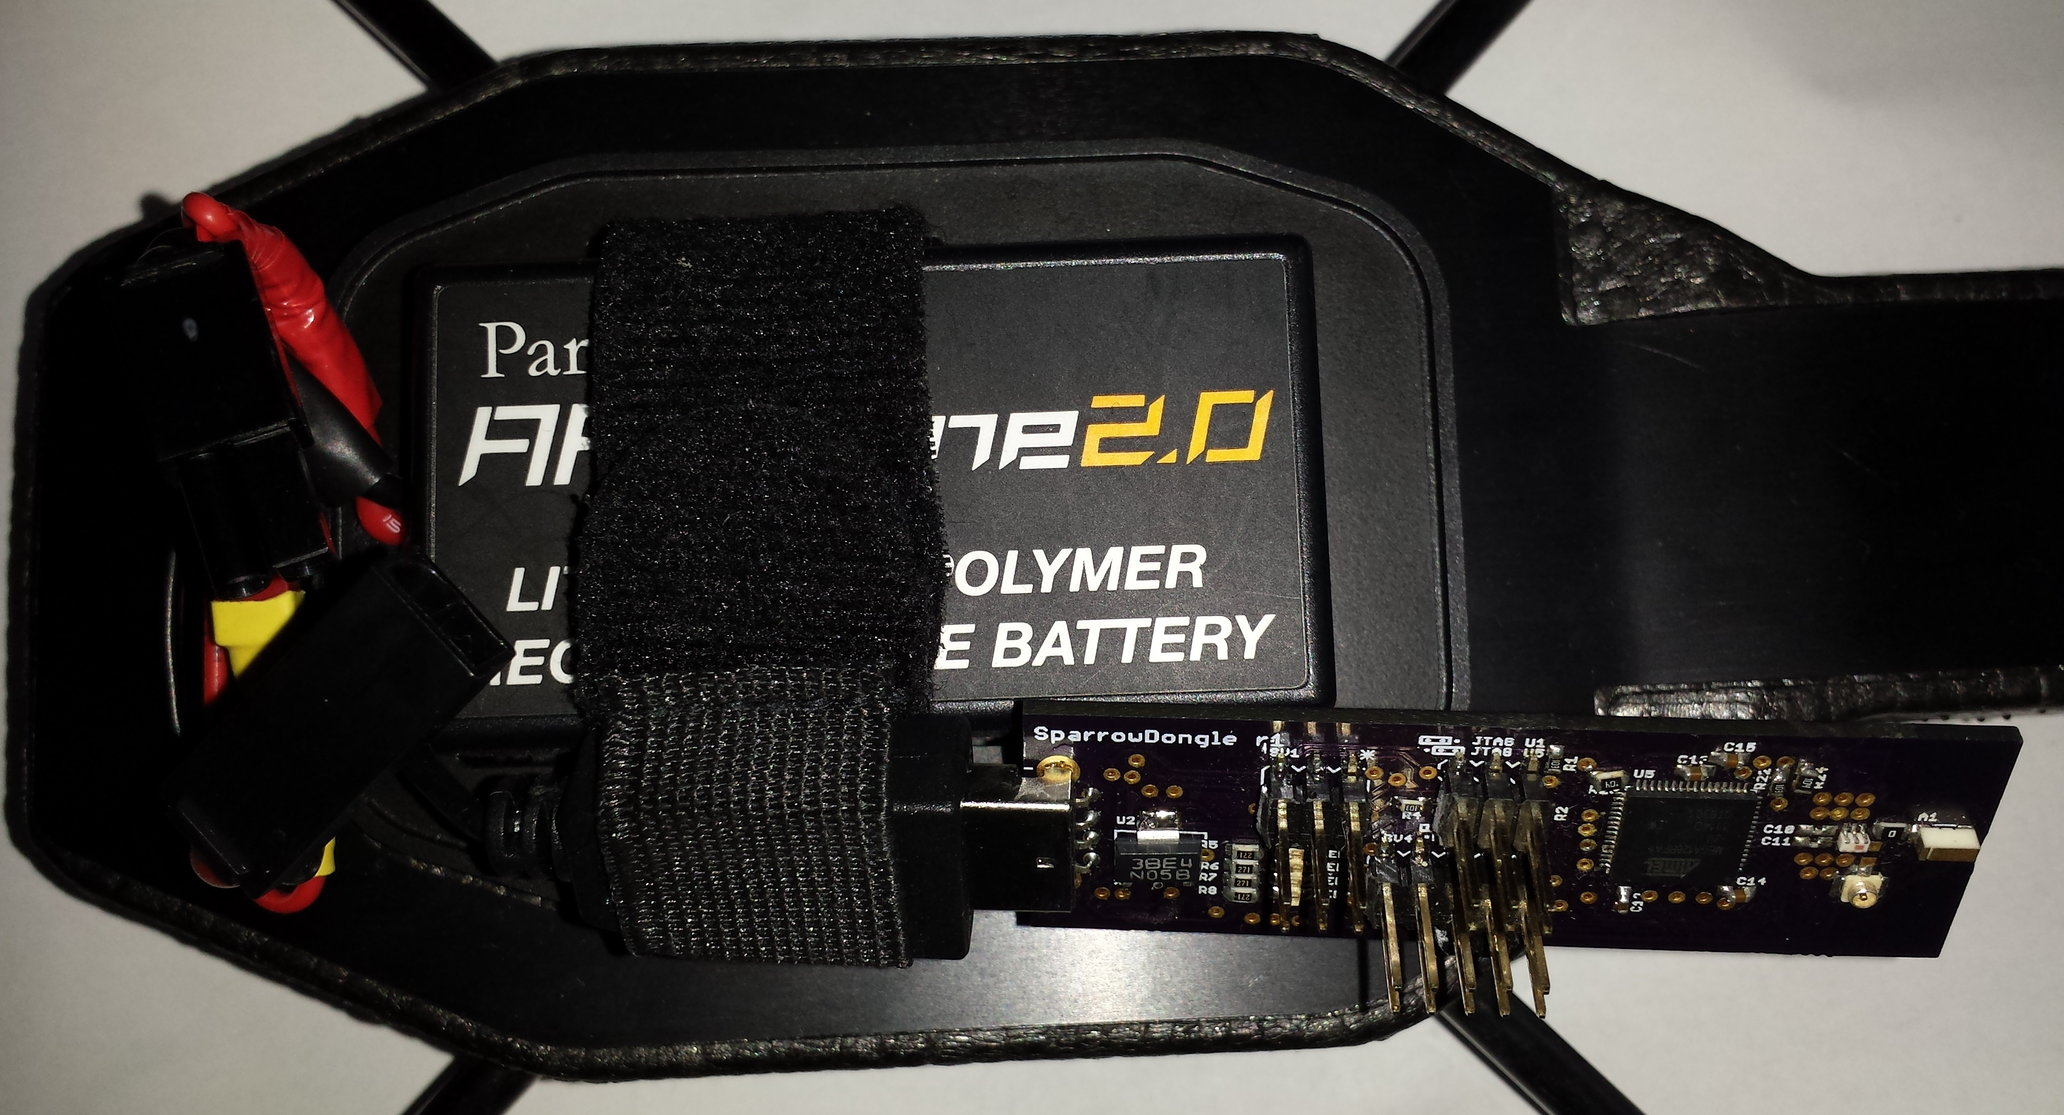
\includegraphics[width=0.45\textwidth]{img/dronedongle.jpg} \caption{SparrowDongle connected to AR Parrot Drone 2.0 } \end{figure}




\section{Related work}
\label{sec:relatedwork}
Even though graph embedding and diagram drawing is a popular subject which has been the topic of articles and research, 
actual open source software which can do such operations is scarce. Algorithms which solve embedding problems have been 
described and implemented since the year 1970. The major impediment for any application which would like to perform 
diagram drawing is actually the diversity and ambiguity of the problem. Apart from performance analysis (time and 
memory consumption), and corectness of the drawing, any other aesthetic appreciation of the result is subjective.
Depending on who the diagram is addressing and which its final scope is, certain styles, connections and layouts are 
appropriate, while others render the final result unasable.

This does not mean that a middle-ground approach does not exist and there are no techniques or conventions which are 
generally accepted as good practice. There are two commonly used open source libraries which provide support for 
drawing diagrams: Graphviz dot\cite{graphvizrelwork} and Eclipse GEF\cite{eclipsegefrelwork}.

\section{Graphviz dot}

\emph{Graphviz dot} is, as described by their own documentation, a command line tool which draws directed graphs as 
hierarchies. It reads its information from text files written in the DOT language and outputs the drawing in 
graphic formats such as GIF(Graphics Interchange Format), PNG(Portable Network Graphics), SVG(Scalable Vector 
Graphics) or PDF(Portable Document Format).

The DOT language input file specifies general information describing the graph. It accepts the definition of three 
main objects: graphs, nodes and edges. A simple graph is described only by its name and a list of nodes and edges.
If the user desires, subgraphs can be defined inside the graph with distinctive characteristics and properties. 
The same can be done for nodes and edges.

\begin{lstlisting}[caption={Simple dot file format}]
digraph G {
	A -> B -> C;
	A -> D;
	A -> E;
	C -> F;
	C -> G;
	D -> F;
	A -> G;
	C -> H;
}
\end{lstlisting}

In terms of implementation, \emph{dot} uses methods such as force directed placing to layout its graphs. Also, its 
layout algorithm presumes graphs are acyclical. This is why dot ensures that all cycles are removed from a graph 
before sending it to the layout routine. 

\begin{lstlisting}[caption={Customized graph dot file representation}]
digraph G {
	size ="4,4";
	main [shape=box]; /*this is a comment*/
	main -> parse [weight=8];
	parse -> execute;
	main -> init [style=dotted];
	main -> cleanup;
	execute -> { make_string; printf}
	init -> make_string;
	edge [color=red]; // so is this
	main -> printf [style=bold,label="100 times"];
	make_string [label="make a\nstring"];
	node [shape=box,style=filled,color=".7 .3 1.0"];
	execute -> compare;
}
\end{lstlisting}

As user-oriented features, the drawings can be manipulated and customized by the user either from a graphical 
interface or by directives specified in the DOT input file. A few examples of such features are: setting dimensions 
and clearance values for node positioning, specifying the direction of edges, label nodes, creatint hyperlinks.

Since it is a command line tool, dot can be integrated with many applications and development environments. From 
custom applications to IDEs, various implementations can use this tool as a means to support drawing diagrams. The 
only requirement is that such an application posseses a means to generate the dot configuration file.

\begin{figure}[ht] \centering
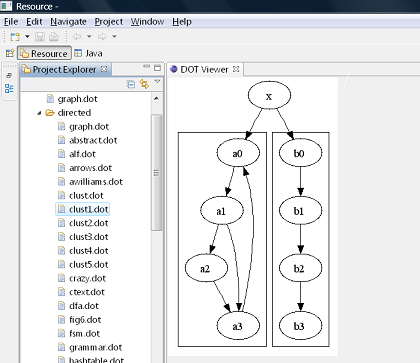
\includegraphics[width=0.45\textwidth]{img/relatedwork/graphviz.png}
\caption{An example of graphviz integrated with the Eclipse IDE.\protect\footnotemark} \end{figure}
\footnotetext{Image taken from \url{http://blog.abstratt.com/}}

\section{Eclipse GEF}

Eclipse GEF(Graphical Editing Framework) provides support for creating graphical editors and views in the Eclipse IDE environment. The graphical 
editors created using GEF allow the user to mainly hand draw any desired graph. All the basic elements required for the task are predefined 
by the underlying library and routing can be performed manually.

Above this basic level, GEF contains classes specialised in layout and connection routing. By default, the library has implementations for 
layout algorithms such as grid layout and tree layout. However, these classes expose API which can be used to create new and more complex 
layout implementations.

\begin{figure}[ht] \centering
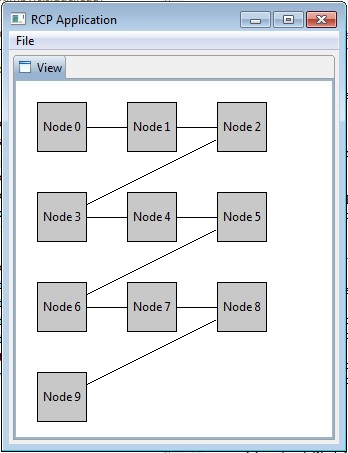
\includegraphics[width=0.35\textwidth]{img/relatedwork/gefexample.jpg}
\caption{Example of a graph viewer implemented using the GEF library.\protect\footnotemark} \end{figure}
\footnotetext{Image taken from \url{http://www.programcreek.com/}}

A notable drawback that GEF presents is the lack of documentation for its API. This may represent a reason why it is not widely 
used, even amongst the Eclipse community. The main sources of information is from articles or community made tutorials, such as 
those of Lars Vogel. Another way of familiarizing oneself with the API and experiencing its capabilities is by running and experimenting 
with the examples suite which comes with the library. These examples showcase typical situations and functionalities step by step through 
simple widgets. While they are educational and helpful for developers, they require an investment of time in order to understand 
the showcased code and functionality.

An extension of Eclipse GEF is Eclipse Zest, which is a visualization toolkit with implementations for different types of graph 
viewers. In essence, a graph viewer is a layout algorithm which specializes in a certain representation of the graph. As 
specified on their homepage, Zest includes a predefined layout package containing algorithms for the following types of 
layouts: Spring, Tree, Radial and Grid. Zest is open to contributions from the community regarding new types of layouts.
Unlike GEF, Zest is does not give the same amount of liberty regarding the representation of nodes. They are static entities, with 
fewer available customizations. Nodes can contain only minimal decorations such as text and an image. This shows that the emphasis 
of this library is on the layout itself.

\begin{figure}[ht] \centering
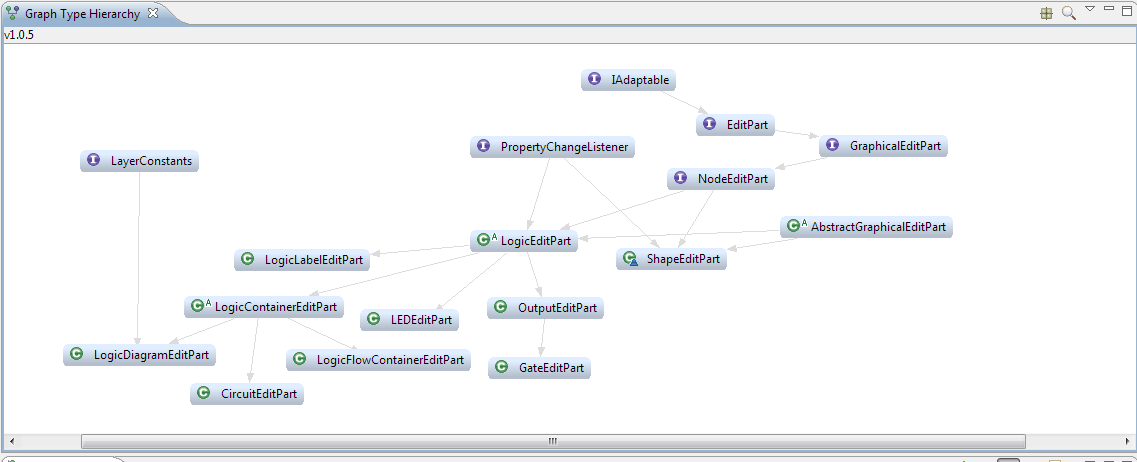
\includegraphics[width=0.85\textwidth]{img/relatedwork/zest.png}
\caption{A graph viewer using Zest radial layout.\protect\footnotemark} \end{figure}
\footnotetext{Image taken from  \url{http://pbwhiteboard.blogspot.ro/}}


\section{System architecture}
\label{sec:architecture}
\label{chap:arch}

\begin{figure*}[ht] \centering
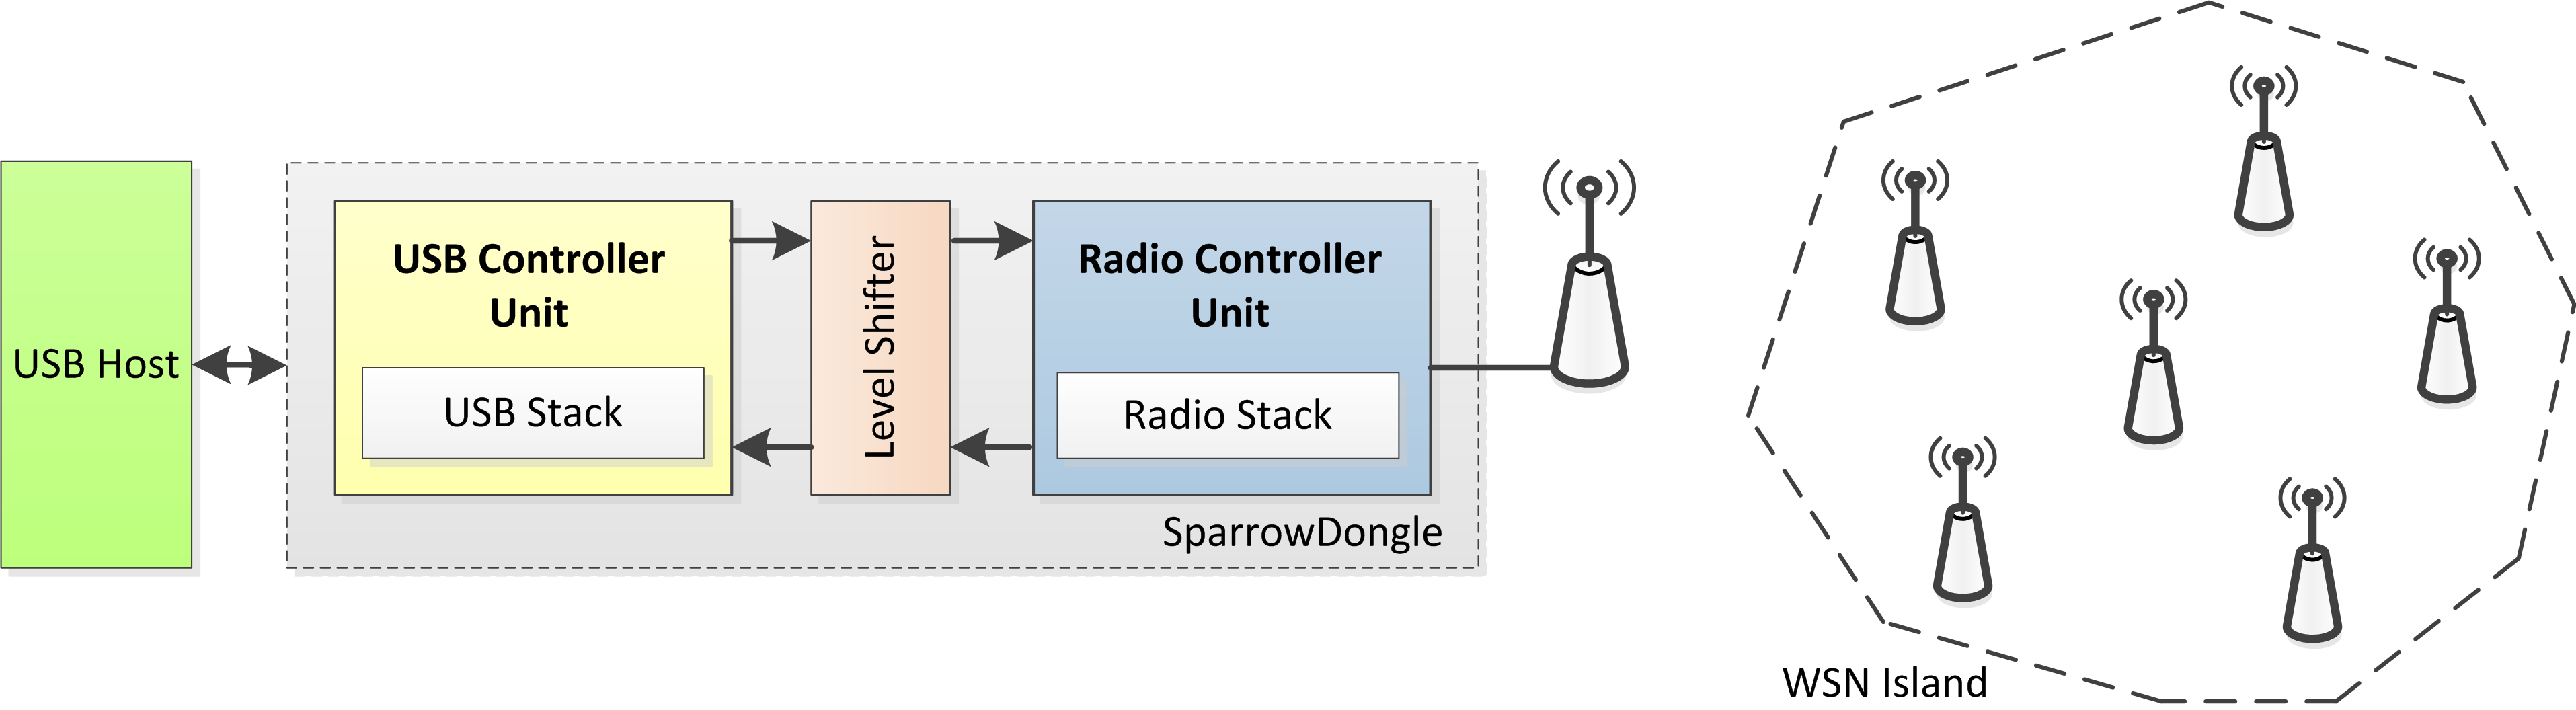
\includegraphics[width=0.9\textwidth]{img/Architecture.png}
\caption{SparrowDongle stick architecture} \end{figure*}

Te classic way of implementing a gateway is by using stationary devices or mobile devices like laptops or phones connected to at least one wireless node. The problem with this type of mobile devices is that you have to be in close proximity of the node in order to communicate with it. This might not be a problem if the nodes are easily accesible, but if a node is situated at a high altitude or over a clif, or even at an unknown location, using drones seems to be the best alternative.

Having this to say, our design has a number of features useful in everyday interaction with a wireless node outlined in \ref{sec:inter},\ref{sec:prox}. 

They can be launch from anyware, fly to any place a node might be placed and gather all the information collected by the nodes.

Additionally, a number of design features were included for ease-of-use in
research and development, outlined in \ref{sec:eng},\ref{sec:data}.


\subsection{\textit{Ease of interaction}} 

\label{sec:inter}

The drone automaticaly detects and initiates a comunication with a nearby node. It searches permanently for any signal emited by a node and sends an ack back to it when it receives any signal. After this first handshake is complet, the node has green light to transmit the information to the gateway installed on the drone. If a node has been detected, the pilot is informed of its presence and if the data transaction completed succesfuly so that he may continue in the search for another node.

\subsection{\textit{Proximity function}} 

\label{sec:prox}

The SparrowDongle can supply informations regarding the nearby nodes by reading the strength of the received signal. Using this information, the pilot can direct the drone closer to the nodes location, either for a faster transfer or to find its exact location. 

Besides the signal strength offered by the SparrowDongle, the drone features an onboard camera with a resolution of 1280x720 pixels streaming at 30 fps. This is very useful in determining the exact location of a wireless sensor node.


\subsection{\textit{Energy Saver}} 

\label{sec:eng}

Due to the comunication protocol implemented, the SparrowV3.2 node uses very little power when not connected to the drone. It broadcasts just a small packet at fixed intervals for low consumtion, and enters on a high bandwith mode when it detecs the presence of a drone for a fast data transfer. 


\subsection{\textit{Latest Data}} 

\label{sec:data}

The data is stored on the flash microcontroller of the node. In this way, the data is persistent in the memory even the power drops and can be recovered when the power is restored. When the memory is full, the oldest data is deleted in order to make space for new one. The data sent to the drone is from the oldest to the newest, so that in the event of a connection lost the node has free space for new data. 



\ref{fig:progr}.


\begin{figure}[ht] \centering \label{fig:progr}
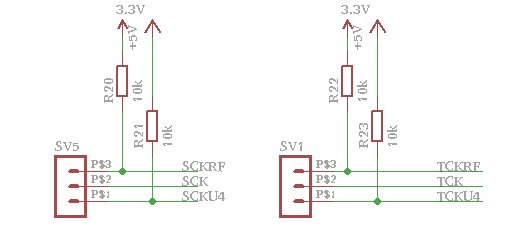
\includegraphics[width=0.35\textwidth]{img/progr.png} \caption{Header selection
for programming clock signals} \end{figure}





\section{Implementation}
\label{sec:implementation}
\label{chap:impl}

\subsection{Placing Algorithm}
 
The placing algorithm is at its core a genetic algorithm \cite{back1997handbook} which uses
a specified set of heuristic functions to compute the fitness of individuals.
An individual is represented by the configuration of the graph at a certain, i.e.
the location of each node.

The idea behind the algorithm is to try and place the graph in a natural way, similar
to how a human would do it by hand. Because every person prefers a different type of 
layout or arrangement, the placing algorithm uses constraints specified by the user
to verify if the graph has been properly placed.

The algorithm starts by creating a generation composed of individuals which have 
been randomly placed on the canvas. It then proceeds to check how good each 
individual is by computing its fitness. This will yield a subset of layouts which
are the closest aproximation of what the user desired. At this point, for each 
part of individual (i.e. a node) it further computes a score, depending on the
number of connections and where it has been placed. Then, two individuals are 
picked and a recombination will be performed. Four new individuals shall be obtained:
one which has the best positions from both parents, one which has the worst positions
from each parent and the last two which have the best from one parent and the 
worst from the other, and vice-versa.

At the end of recombination, a new generation will have been obtained. This selective 
evolution process \cite{back1996evolutionary} will continue until either stability has been achieved (there is an
individual with the best fitness which appears constantly in every generation) or, for 
performance reasons, a certain number of generations has passed. The individual with 
the best fitness shall represent the final layout.

\subsection{Routing Algorithm}

The routing algorithm is based on the orthogonal edge routing. This method ensures 
that all the edges which compose a connection path are orthogonal. Also, another 
imposed restriction is that, when possible, no path should cross another path to 
avoid creating confusing intersection points.

The algorithm mixes a shortest path approach with an original take on avoiding obstacles.
At first, in order to route a path, the shortest path between the two components that have 
to be connected is computed, ensuring that it avoids obstacles. Then, all redundant points 
are eliminated (a redundant point is any point C which is on a valid segment [AB]). After 
this step, the path is "orthogonalized", meaning that all edges which are not orthogonal are 
broken into smaller, orthogonal edges. Should any of these new segments intersect an obstacle,
that segment shall be treated as a separate route and re-computed so that it no longer 
intersects the obstacle.

Should the computed path intersect any other already existing path, a new one shall be 
computed. It will no longer be the shortest, but it will trade area covered by the drawing 
for clarity and better understanding of the graph.

\begin{figure}[ht] \centering
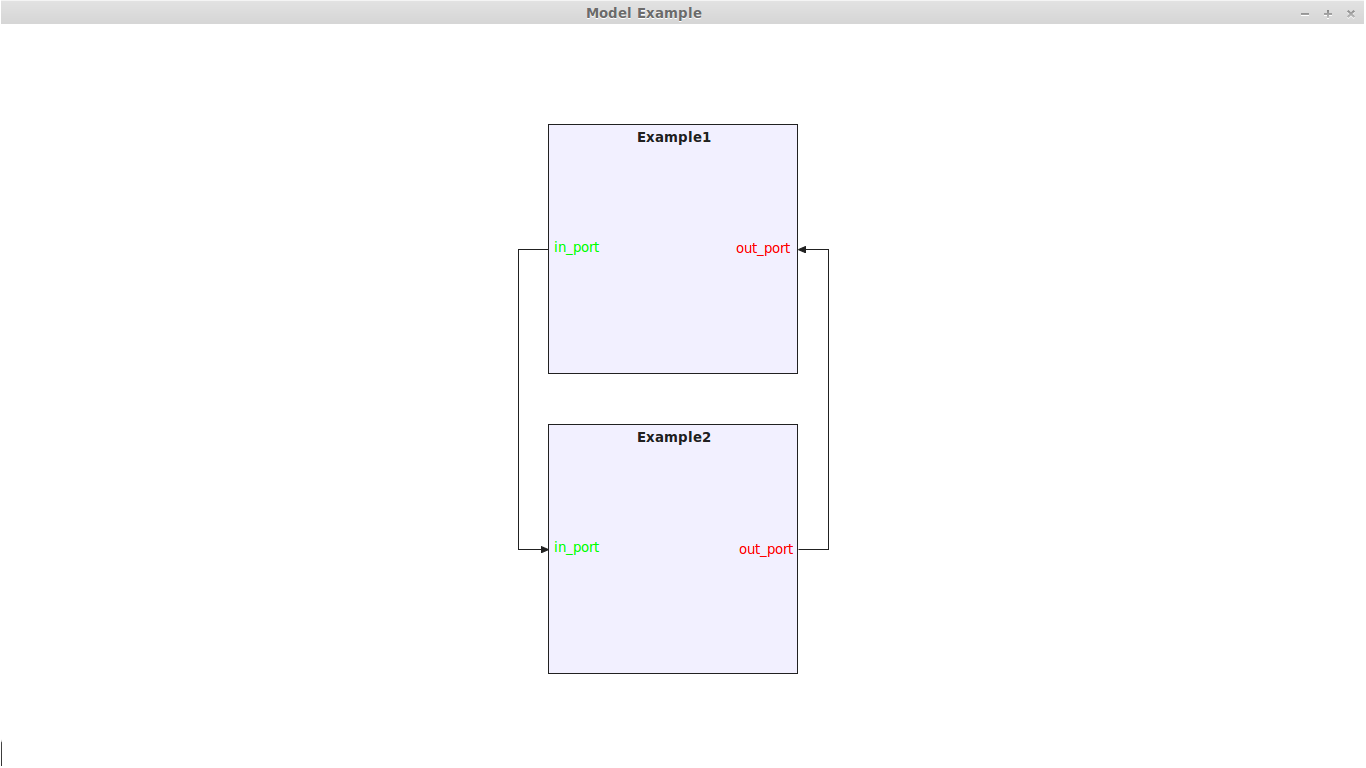
\includegraphics[width=0.5\textwidth]{src/modelExample.png}
\caption{The general look of nodes and routes in the model. Input ports are highlited green; output ports are highlighted red; arrow decorations are placed 
at the end of a route to show its direction.} \end{figure}



\section{Results} 
\label{sec:results}
\label{chap:results}

In this chapter we will cover the results obtained with this gateway platform
and other possible applications.

\begin{figure}[ht] \centering
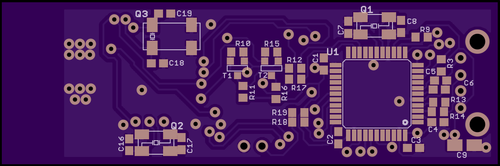
\includegraphics[width=0.3\textwidth]{img/dongleb.png} \caption{Bottom side of
SparrowDongle PCB} \end{figure}


\begin{figure}[ht] \centering
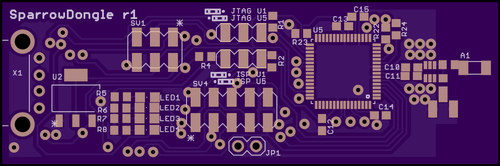
\includegraphics[width=0.3\textwidth]{img/donglef.png} \caption{Top side of
SparrowDongle PCB} \end{figure}

\subsection{Performance}

Throughput testing was done with back-to-back packets sent at 250kbps over
2.4GHz with one sending node in acceptable range, with no losses. This is due
to the double-buffering used in receiving packets from the wireless network.
As soon as one packet ends, a signal is sent to the radio controller unit with
a small delay of 9$\mu S$. Even if a new packet starts in that small interval,
receipt of the new packet goes unhindered as the first bytes of the old packet
have already been transfered to a different memory location from which they
will be sent to the USB controller unit via the serial connection.

\subsection{Software configurations}

A great advantage of using a dedicated USB Controller Unit for the gateway is
that it can be programmed as one of several USB Communication Classes. The USB
Controller Unit is not limited in implementing any of these classes since most
of the computing power at its disposal is reserved for USB.  SparrowDongle can
appear as different USB devices:

\begin{itemize}

\item \textit{Virtual Serial Port}: Communication with the wireless island
around the gateway can be made via a serial link, incoming packets will appear
on the receive end of this port and packets will be sent on the transmit end.
In typical Unix fashion, our implementation sends packet in ASCII for ease of
use and debugging. They are converted to binary form on the Radio Controller
Unit of the gateway

\item \textit{Ethernet Emulation}: In this fashion, packets are received on the
gateway and then encapsulated in an Ethernet packet sent over the USB link
(Ethernet is emulated between the USB device and USB host)

\item \textit{Network card}: SparrowDongle behaves as a wireless network card,
the operating system will register a network interface for the gateway and
addresses assigned to this interface will change the gateway's address in the
wireless medium (as opposed to changing the address for the emulated Ethernet)

\item \textit{Mass Storage}: SparrowDongle can offer a virtual filesystem
interface for innovative data acquisition from the wireless sensor network. In
accordance with the Unix philosophy of "everything is a file", the virtual
filesystem offered by the USB stick could have a file for each wireless node
where it stores recent data (as much as the gateway can store in its volatile
memory, 1-2 records per node). The software implementation for this interface
is under development.

 \end{itemize}

\subsection{Applications}


The versatility of the SparrowDongle gateway platform allows it to be deployed
in a wide range of applications, whether the gateway has to be connected to a
PC or a small embedded device, whether it has to implement a virtual serial
connection or to emulate an ethernet link.

For instance, these are the application in which SparrowDongle is currently
deployed:

 \begin{itemize} 

\item Collecting data from the sensors \cite{fcint}

\item Debuging a wireless sensor network by checking which node is working, the connection logs and the physical state of the device

\item Search and rescue operations, especialy when going skiing in a avalanche prone enviroment by wearing a wireless sensor. 

\item Creating a small wireless sensor network for a limited time with small costs and large battery life

\item Treasure hunt where the sensors can hold the clues that lead to the location of the treasure
 
\end{itemize}



\section{Conclusion}
\label{sec:conclusion}
The paper presented a routing algorithm which uses newer algorithms and
programming techniques to achieve results which are more pleasant for the
user. In addition, it is easily customizable to meet the needs and 
preferences of any user.

The algorithm clearly separates its two functionalities, allowing the 
user to customize whichever algorithm feels unsuitable, making the 
final diagrams feel more natural and easily understandable.


\bibliographystyle{abbrv}
\bibliography{orthogonal-routing}

\end{document}
